\section{Accumulated Muon Deflection}\label{sec:accum_defl}

As shown in Section~\ref{sec:defl_per_int}, the deflection per interaction 
is lower $\SI{1}{\degree}$ and thus not relevant for the current muon 
directional reconstruction. Since these deflections accumulate along the 
propagation distance, the angle between the incoming muon and the outgoing 
muon direction is simulated. 
At first, the deflections in PROPOSAL are compared to 
the tools MUSIC and GEANT4.



\begin{figure}
    \centering
    \subcaptionbox{
        \label{fig:compare_MUSIC_degree}}
        {\includegraphics[width=0.48\textwidth]{figures/compare_MUSIC_degree.pdf}}
    \subcaptionbox{
        \label{fig:compare_MUSIC_dist}}
        {\includegraphics[width=0.48\textwidth]{figures/compare_MUSIC_dist.pdf}}
    \caption{}
    \label{fig:compare_MUSIC}
\end{figure}








For current analyses, it is important to study the impact of the muon 
deflection on the angular resolution to estimate a reconstruction uncertainty.
For this purpose, four different initial energies 
from $E_{\text{i}} = \SI{10}{\tera\electronvolt}$ to 
$E_{\text{i}} = \SI{10}{\peta\electronvolt}$ are used and the final 
energy is set to $E_{\text{f,\,min}} \geq \SI{10}{\giga\electronvolt}$ with 
$E_{\text{f,\,min}} < E_{\text{i}}$ for each simulation. To compare the results of 
a total of $\num{36}$ simulations, the median of the deflection distribution 
with a $\SI{95}{\percent}$ central interval is presented in 
Figure~\ref{fig:fit_median}.

\begin{equation}
    \label{eqn:fit_median}
\end{equation}


\begin{figure}
    \centering 
    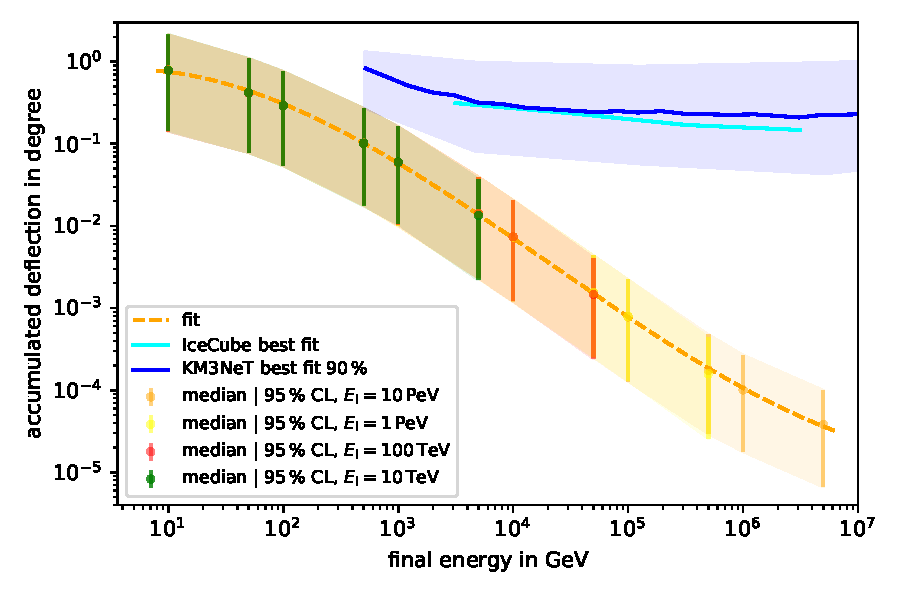
\includegraphics[width=0.8\textwidth]{figures/fit_median_defl_cut_10percent_only_poly.pdf}
    \caption{The median of the accumulated deflection with a $\SI{95}{\percent}$ 
    central interval is shown for four different initial energies $E_{\text{i}}$. 
    Each data set includes more than $\num{50000}$ events with the requirement 
    that the true final particle energy $E_{\text{f}}$ is maximum 
    $\SI{10}{\percent}$ below the set final energy $E_{\text{f,\,min}}$,   
    $E_{\text{f}} > E_{\text{f,\,min}} \cdot 0.9$. The energy cuts are $\texttt{e\_cut} = \SI{500}{\mega\electronvolt}$ and $\texttt{v\_cut} = 0.05$. 
    Since the medians overlap for different initial energies, there is no 
    strong impact of the initial energy on the median deflection. These 
    medians can be fit by a third degree polynomial in the log-space as 
    shown in Equation~\ref{eqn:fit_median}. For energies 
    $E_{\text{f}} \approx \SI{500}{\giga\electronvolt} - \SI{1}{\tera\electronvolt}$, there is a minimal influence of deflection on the angular resolution of 
    KM3NeT \cite{KM3NeT_Resolution2016}. The resolution of IceCube is not 
    impacted \cite{IceCube_Resolution2021}.}
    \label{fig:fit_median}
\end{figure}